\documentclass{article}
\usepackage{geometry}
\geometry{a4paper, margin=1in}
\usepackage{booktabs}
\usepackage{array}
\usepackage{amsmath}
\usepackage{physics}
\usepackage{graphicx}
\usepackage{xcolor}
\usepackage{multirow}
\usepackage[labelfont=bf]{caption}
\usepackage{graphicx}
\graphicspath{{picture/}}

\usepackage{subcaption}  % for subfigures
\usepackage{float}       % for [H] placement
\usepackage{hyperref}   % for hyperlinks
\usepackage{cleveref}   % for \cref and \Cref references

\usepackage[backend=biber,style=ieee,doi=true,url=true]{biblatex}
\addbibresource{refs.bib}


\title{Performance Evaluation of Track Matching between the Muon Forward Tracker and Muon Chambers in the ALICE Experiment}
\author{Haidar Reslan \\ \small Supervised by: Batoul Diab}

\date{  \today
        \\ \small CERN Summer Student Programme 2024} 
      


\begin{document}

\maketitle

\begin{abstract}
This work \footnote{The analysis code is available at: \url{https://github.com/haidaara/ALICE-O2-forward-track-analysis}}evaluates the performance of track matching between the Muon Forward Tracker (MFT) and the Muon Chambers (MCH) in the ALICE experiment.
Monte Carlo simulations were used to calculate efficiency and purity, both in integrated form and differentially as functions of transverse momentum,
azimuthal angle, pseudorapidity, matching $\chi^2$, and the number of MFT clusters.

The integrated performance shows an efficiency of about 75\% and a purity of about 45\%. Differential studies indicate that efficiency
is generally stable across most variables, while purity is more sensitive, particularly at low $p_T$ and for looser $\chi^2$ selections.\
A scan of the $\chi^2$ threshold identified an optimal working point near $\chi^2 \approx 20$, which provides the best balance between 
efficiency and purity.

Although the sample size was limited, leading to larger statistical uncertainties in some regions, the results confirm the robustness 
of the matching method and provide a basis for future studies.
\end{abstract}


\section{Introduction}
\subsection{Physics Motivation}
Heavy-flavor particles such as quarkonia (J/$\psi$, $\Upsilon$) and open heavy-flavor mesons (D, B) are valuable probes of the hot, dense matter created in heavy-ion collisions.
These particles predominantly decay into muon pairs in the forward rapidity region. In run 3, an interesting challenge is the precise reconstruction of such di-muon 
events between the vertexing detector (MFT) and the muon spectrometer (MCH--MID). For precise vertexing and pointing, we match MFT space points 
to MCH-MID muon tracks.
The presence of a hadron absorber further complicates this task by introducing multiple scattering and energy loss, making the matching process both 
physically and technically challenging.


\subsection{Track Matching Challenge}
The track-matching problem is complex. High-multiplicity events generate a large combinatorial background, where thousands of charged tracks produce fake associations. In addition, the MFT provides precise space points near the vertex, while the spectrometer measures muon trajectories and momenta downstream of the absorber. Finally, propagation across detectors introduces uncertainties from multiple scattering, material effects, and possible misalignments when extrapolating tracks to a common reference plane.

A complete methodology for addressing this problem must combine several elements:

\begin{itemize}
    \item \textbf{Coordinate transformations} between MFT and MCH parameterizations;
    \item \textbf{Candidate selection};
    \item \textbf{Best-match identification} using $\chi^2$ minimization;
    \item \textbf{Covariance propagation} to incorporate detector uncertainties;
    \item \textbf{Timing information} to suppress fake matches in high-occupancy events;
    \item \textbf{ML detection} to optimize the efficiency--purity balance.
\end{itemize}

\subsection{Detector System Type and Description ``ALICE Muon Arms''}
The ALICE experiment is featured by a dedicated forward muon spectrometer that covers the pseudorapidity range $-4.0 < \eta < -2.5$. This spectrometer integrates three complementary
subsystems aligned along the beam axis, each designed to address specific tasks including precise vertex determination, momentum measurement, and muon identification.

The \textbf{Muon Forward Tracker (MFT)} is positioned upstream of the absorber ($z \approx -45$ to $-65$ cm), covers the pseudorapidity range $-4.0 < \eta < -2.5$.
This silicon pixel detector provides high-precision space points close to the interaction vertex, with spatial resolution of $\sigma_{xy} \approx 5 \mu$m and momentum
resolution of $\Delta p_{\text{T}}/p_{\text{T}} \approx 20\%$ at 10 GeV/c. Its primary function is to provide the muon spectrometer with access to the vertex information,
which is crucial for rejecting background muons from hadron decays.

Located between the MFT and MCH ($z \approx -90$ to $-500$ cm), the \textbf{Front Absorber} consists of carbon, steel, and concrete layers. 
This component filters out hadrons while allowing muons to pass through, effectively reducing background contamination. However, it introduces multiple scattering effects 
that must be carefully accounted for in the track matching process.

Downstream of the absorber ($z \approx -500$ to $-1000$ cm), the \textbf{Muon Tracking Chambers (MCH)} cover the same pseudorapidity range as the MFT. 
These ten stations of cathode pad chambers provide precise momentum reconstruction in the 0.2 T dipole field, with momentum resolution of $\Delta p_{\text{T}}/p_{\text{T}} 
\approx 1\%$ at 10 GeV/c and spatial resolution of $\sigma_{xy} \approx 100 \mu$m. The MCH measures particle trajectories after they have passed through the absorber.

At the spectrometer end ($z \approx -1400$ cm), the \textbf{Muon Identifier (MID)} utilizes resistive plate chambers to tag muons based on their penetration depth. 
This system effectively rejects hadrons and provides the trigger signal necessary for identifying muon events.

It is important to note that a coordinate transformation is required between the MFT and MCH systems, as each employs its own parameterization system. 
Transformation equations have been established to facilitate accurate matching between these detector components.
Noting also that a coordinate transformation is needed as each of MFT and MCH has its parameterization system, so transformation equations are established between them.

\begin{figure}[htbp]
    \centering
    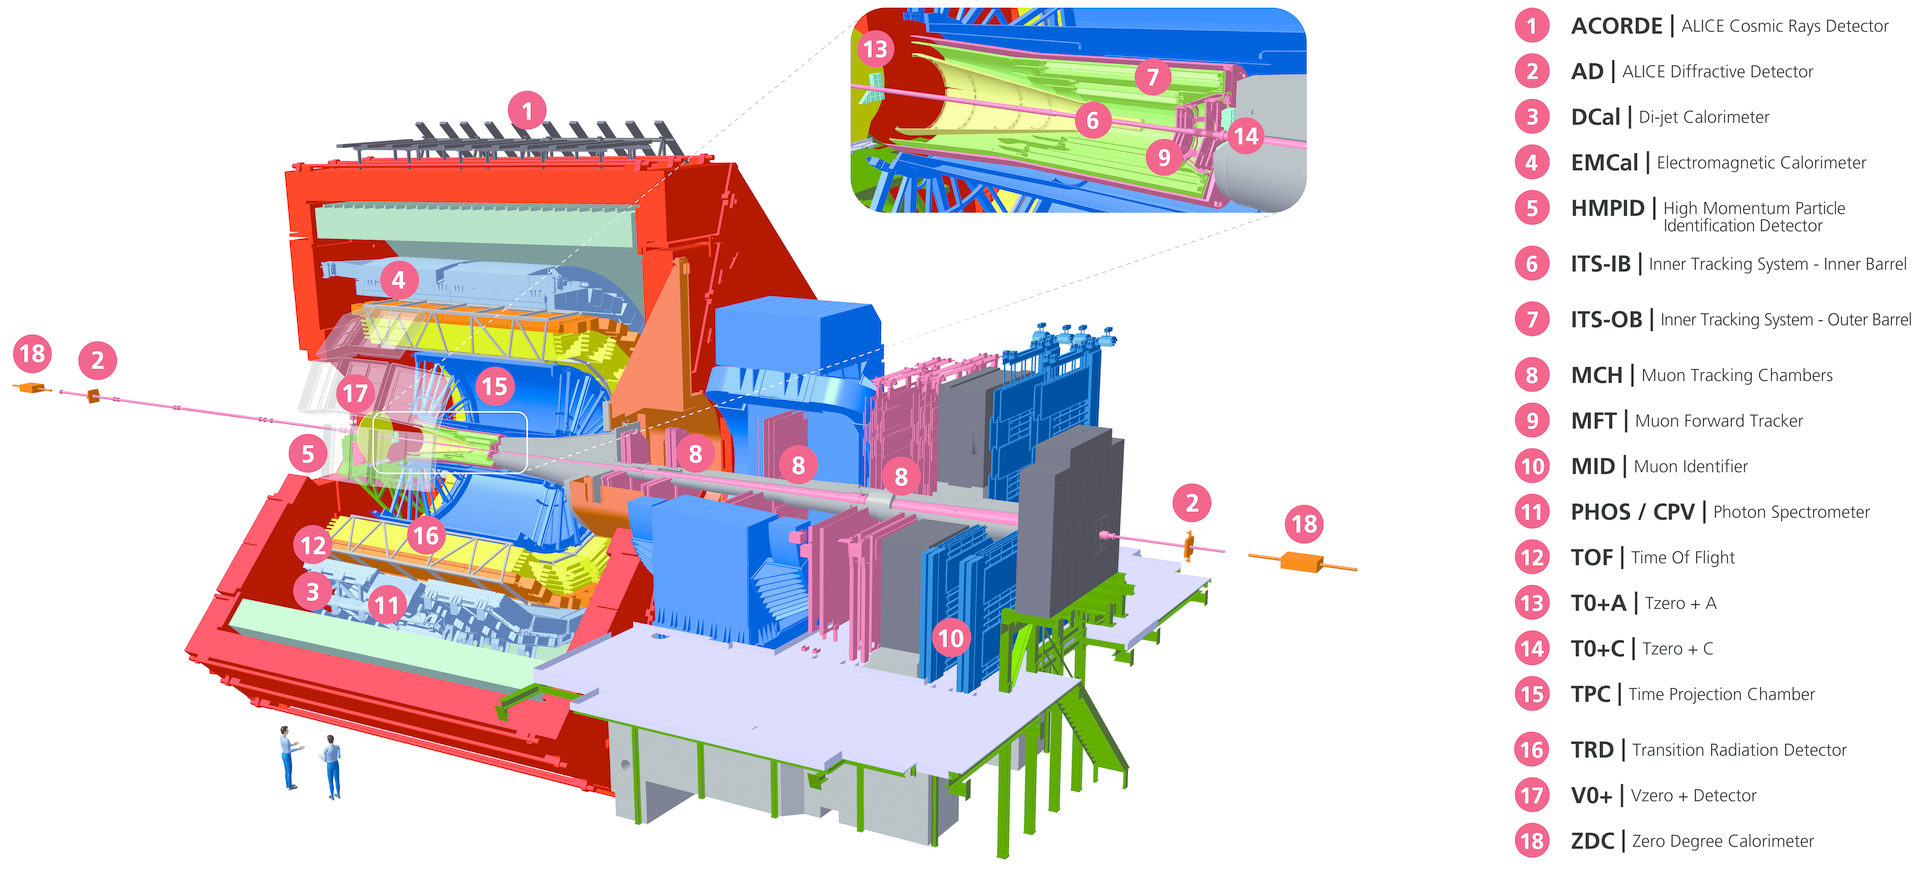
\includegraphics[width=1\textwidth]{picture/alice_detector.png}
    \caption{Overview of the ALICE detector \cite{ALICE_DetectorFig} in it's Run 3}
    \label{fig:Alice_Detector}
\end{figure}

\emph{note: to Batoul } is it better to have this section as compacted paragraph or like before as bullet point?  


\subsection{Track Type}
ALICE categorizes muon tracks based on detector contributions. The core objective of the matching algorithm is to convert Type 3 tracks (standalone muons) into Type 0 tracks (global muons) by correctly associating them with an MFT track.

\begin{table}[h]
\centering
\caption{ALICE Muon Track Classification}
\label{tab:track_types}
\begin{tabular}{clll}
\toprule
\textbf{Type} & \textbf{Classification} & \textbf{Components} & \textbf{Key Characteristics} \\
\midrule
\textbf{0} & Global Muon & MFT + MCH + MID & Full reconstruction with vertex and momentum; successful match between MFT and MCH--MID \\
\textbf{2} & MFT-MCH Track & MFT + MCH & No muon identification (MID missing) \\
\textbf{3} & Standalone Muon & MCH + MID & Spectrometer-only reconstruction; candidate for matching to MFT \\
\textbf{4} & MCH Track & MCH only & MCH only reconstruction \\
\bottomrule
\end{tabular}
\end{table}

\subsection{AOD Branch}
\textbf{The Essential used branches for matching analysis:}\\
Although the AOD contains many branches, only a small subset is essential for matching analysis. These govern the kinematics, classification, matching quality, and truth validation:

\begin{table}[h]
\centering
\caption{Essential AOD Branches for Matching Analysis}
\label{tab:aod_branches}
\begin{tabular}{>{\raggedright\arraybackslash}p{3cm}>{\raggedright\arraybackslash}p{3cm}ll}
\toprule
\textbf{Category} & \textbf{Branch} & \textbf{Type} & \textbf{Description} \\
\midrule
Kinematics & \texttt{fX, fY, fZ} & Float & Position at reference plane (cm) \\
& \texttt{fPhi} & Float & Azimuthal angle (rad) \\
& \texttt{fTgl} & Float & tan$\lambda$ (dip angle tangent) \\
& \texttt{fSigned1Pt} & Float & q/$p_{\text{T}}$ (GeV/c)$^{-1}$ \\
\midrule
Classification & \texttt{fTrackType} & Int & 0/2/3/4 track category \\
\midrule
Matching & \texttt{fChi2MatchMCHMFT} & Float & $\chi^2$ of MFT-MCH candidate \\
& \texttt{fIndexMFTTracks} & Int & Index of matched MFT track \\
\midrule
Truth (MC) & \texttt{fMcMask} & UInt & MC truth bitmap (bit 7 = muon, bit 8 = prompt) \\
\bottomrule
\end{tabular}
\end{table}

\subsection{Monte Carlo Simulation and Event Generation}
The analysis utilizes Monte Carlo (MC) simulated events to provide the ground truth information essential for evaluating track matching performance. The simulation chain includes:

\begin{itemize}
    \item \textbf{Event Generator:} Pythia 8 is used for proton-proton collision event generation, with specific configuration for prompt J/$\psi$ production and decay into muon pairs.
    
    \item \textbf{Detector Simulation:}
    \begin{itemize}
        \item GEANT3/GEANT4 simulation package models the passage of particles through the ALICE detector material
        \item Includes detailed description of the muon spectrometer geometry, materials, and magnetic field
        \item Simulates energy loss, multiple scattering, and secondary particle production
    \end{itemize}
    
    \item \textbf{MC Truth Information:}
    \begin{itemize}
        \item Each reconstructed track is associated with its generated MC particle through the \texttt{fMcMask} branch
        \item Bitmap encoding provides information about particle origin and properties:
        \begin{itemize}
            \item Bit 7: Identifies muons
            \item Bit 8: Flags prompt particles (not from decay chains)
        \end{itemize}
        \item Value of 0 indicates a perfect match to a generated muon
        \item Value of 127 indicates a false match
    \end{itemize}
    
    \item \textbf{Simulation Parameters:}
    \begin{itemize}
        \item Events generated at $13$ TeV center-of-mass energy
        \item Includes full simulation of the absorber material effects and multiple scattering
        \item Accounts for detector alignment uncertainties and resolution effects
    \end{itemize}
\end{itemize}

The use of MC simulation enables the precise definition of efficiency and purity, as the true particle identity and origin are known for each reconstructed track, allowing for unambiguous performance evaluation of the matching algorithm.

\emph{note: to Batoul } is it better to have this section as compacted paragraph or like before as bullet point?  


\section{Analysis Methodology and Software Framework}

\subsection{File Organisation}
The analysis is built on a ROOT-based framework. The core class, \texttt{O2fwdtrack}, is automatically generated from the TTree structure.

\begin{itemize}
    \item \texttt{O2fwdtrack.h}: Contains the class definition, data structures, and function declarations.
    \item \texttt{O2fwdtrack.C}: The main file containing the \texttt{Loop()} function. The core functionality is divided into two main parts:
    \begin{itemize}
        \item Plotting available branches by invoking basic helper functions for branch variables
        \item Invoking efficiency/purity calculation through the \texttt{CalculateEfficiencyPurity()} function
    \end{itemize}
    \item \texttt{O2fwdtrackEfficiency.C}: Contains the core logic for efficiency/purity calculation within \texttt{CalculateEfficiencyPurity()}. All other related functions are invoked from within this function.
    \item \texttt{O2fwdtrackGraphing.C}: Handles all visualization and results extraction via the \texttt{ReportAndOptimize()} function.
    \item \texttt{O2fwdtrackHelpers.C}: Provides utility functions for initializing, filling, and plotting basic histograms of track variables.
\end{itemize}

\subsection{Function Hierarchy and Workflow}
As mentioned in Section 3.1, the implementation consists of two main functional parts. The first part handles basic histogram operations for the \texttt{O2fwdtrack} branch different variable: initializing histograms, filling them with branch variable entries, and plotting the results. The second part, which is the focus of this analysis, deals with efficiency and purity calculations, primarily orchestrated by the \texttt{CalculateEfficiencyPurity()} function.

The efficiency/purity analysis follows a structured workflow consisting of several specialized functions:

\begin{enumerate}
    \item \textbf{Main Orchestration (\texttt{CalculateEfficiencyPurity()})}: Coordinates the entire efficiency/purity calculation process throughseveral specialized sub-functions called inside it.
    
    \item \textbf{Histogram Creation (\texttt{CreateEfficiencyPurityHistograms()})}: Initializes 1D and 2D histograms for all defined analysis variables but does not fill them with data.
    
    \item \textbf{Candidate Collection (\texttt{CollectMatchCandidates()})}: Iterates through all entries and filters matched tracks. Instead of filling histograms directly, matching entries are stored in a vector of \texttt{MatchCandidate} objects for subsequent processing.
    
    \item \textbf{Best Match Selection (\texttt{SelectBestMatches()})}: For each MCH track, evaluates its candidate matches and selects the one with the smallest \texttt{fChi2MatchMCHMFT} value that falls below the defined threshold (\texttt{fChi2Threshold}). The selected candidates are stored in a \texttt{BestMatch} vector also.
    
    \item \textbf{Histogram Filling (\texttt{FillEfficiencyPurityCounts()})}: Processes entries again to populate denominator and numerator histograms for both efficiency and purity calculations. This function considers track types and utilizes the \texttt{bestMatches} map while also maintaining four essential counters: \texttt{nTotalType3}, \texttt{nMatchedType3}, \texttt{nTotalType0}, and \texttt{nTrueType0}.
    
    \item \textbf{Result Calculation \& Optimization (\texttt{ReportAndOptimize()})}: Computes final efficiency and purity values from the accumulated counters. Performs a comprehensive scan of $\chi^2$ thresholds to identify the optimal value that maximizes the product of efficiency and purity. Finally, invokes graphing functions to generate all output visualizations.
\end{enumerate}

The latter two functions implement sophisticated filling and reporting methodologies based on the precise definitions of efficiency and purity ratios, which are elaborated in the following section.

\subsection{Definition of Efficiency and Purity}
The analysis uses the following rigorous definitions, which directly dictate the histogram filling logic:

\begin{itemize}
    \item \textbf{Efficiency ($\epsilon$)}: The probability that a true standalone muon (MCH-MID) track is correctly matched to its true MFT counterpart.
    \begin{itemize}
        \item \textbf{Numerator}: True matched global muons (\texttt{nMatchedType3}). Filled from the \texttt{bestMatches} map for type 3 tracks where \texttt{fMcMask == 0}.
        \item \textbf{Denominator}: All MCH-MID tracks in acceptance (\texttt{nTotalType3}). Filled from all type 3 tracks within $-3.6 < \eta < -2.5$.
        \item \textbf{Formula}: $\epsilon = \frac{N^{matched}_{true\ Type3}}{N^{total}_{Type3}}$
    \end{itemize}
    
    \item \textbf{Purity ($P$)}: The probability that a selected global muon track is a true match, not a combinatorial fake.
    \begin{itemize}
        \item \textbf{Numerator}: True global muons (\texttt{nTrueType0}). Filled from type 0 tracks where \texttt{fMcMask == 0}.
        \item \textbf{Denominator}: All selected global muons (\texttt{nTotalType0}). Filled from all type 0 tracks.
        \item \textbf{Formula}: $P = \frac{N^{true}_{Type0}}{N^{total}_{Type0}}$
    \end{itemize}
\end{itemize}

Based on these definitions, we carefully build the two numerators and two denominators needed for our calculations. As the code runs through different types of tracks in separate steps, it keeps track of four important numbers: \texttt{nTotalType3}, \texttt{nMatchedType3}, \texttt{nTotalType0}, and \texttt{nTrueType0}. 

The respective ratio of these variable - matched Type 3 over total Type 3 for efficiency, and true Type 0 over total Type 0 for purity - we get the final efficiency and purity values that you see reported. What's really useful is that these numbers match up with what we get when we look at the average values from our efficiency and purity plots, which helps confirm that the analysis methodology is internal consistent.

\subsection{Matching Process Implementation}
The matching process utilizes the existing \texttt{fMcMask} branch from the TTree, which provides MC truth information:

\begin{verbatim}
// As implemented in CollectMatchCandidates() and FillEfficiencyPurityCounts()
if (fMcMask == 0) {
    // Identifies true match to generated muon
    // Used to fill efficiency numerator and purity numerator
} else {
    // Indicates background or combinatorial match
}
\end{verbatim}

\section{Results and Discussion}

\subsection{Integrated Performance Metrics}
The integrated performance metrics provide a comprehensive overview of the MCH-MFT track matching algorithm's effectiveness.\\

\textbf{Efficiency:} $\epsilon = 0.754$ \\
\textbf{Purity:} $P = 0.447$

A detailed event count is recorded in the following four variables:
\begin{table}[h]
    \centering
    \caption{Track matching event counts and metrics}
    \label{tab:track_metrics}
    \begin{tabular}{lrrl}
        \toprule
        \textbf{Metric} & \textbf{Value}  & \textbf{Description} \\
        \midrule
        nTotalType3 & 1910 & Total MCH-MID tracks in acceptance \\
        nMatchedType3 & 1441 & Correctly matched true tracks \\
        nTotalType0 & 3345  & Total selected global muons \\
        nTrueType0 & 1496 & True global muon matches \\
        \bottomrule
    \end{tabular}
\end{table}

The integrated efficiency of 75.4\% demonstrates that the algorithm successfully matches approximately three out of every four true muon tracks between the MCH and MFT systems. This indicates generally effective matching capability across the detector acceptance. The purity value of 44.7\% reflects the significant challenge posed by combinatorial background, suggesting that more than half of the selected global muon candidates originate from incorrect matches.

These results clearly indicate potential areas for improvement in future iterations of the matching methodology, particularly in enhancing background rejection while maintaining high efficiency.

\subsection{Differential Metrics}

Beyond the integrated values, the performance of the matching algorithm was studied as a function of several track-level observables. For each observable, efficiency and purity distributions were extracted, allowing us to probe phase-space--dependent effects.

The following variables were considered:

\begin{itemize}
    \item \textbf{Transverse momentum (pT) \cref{fig:var-pt}}
    
    At low transverse momentum ($p_T < 1\ \text{GeV}/c$), the efficiency rises steeply as tracks become easier to reconstruct and match across 
    detectors. In the intermediate $p_T$ region ($2-8\ \text{GeV}/c$), the efficiency stays stable around 80-90\%, indicating robust matching performance.
    However, the purity remains relatively low (10-25\%), reflecting the presence of combinatorial matches in high-multiplicity environments. 
    At high $p_T$, both efficiency and purity exhibit large statistical uncertainty. In particular, the large error bar on the final efficiency 
    point reflects the limited number of muons available in this region of phase space in the simulation, leading to poor statistical precision.

    \item \textbf{Azimuthal angle ($\phi$) \cref{fig:var-phi}}
    
    At most azimuthal angles, the efficiency stays high, usually between 70-85\%. There are some ups and downs across $\phi$, 
    which probably come from the way the detector is segmented or from variations in acceptance. The purity is lower, around 40-50\%, 
    but it stays fairly steady without sharp drops. The error bars are similar across $\phi$, which means the simulation provided enough tracks in 
    all regions, so these results can be trusted.

    \item \textbf{Pseudorapidity ($\eta$) \cref{fig:var-eta}}
    
    The efficiency depends strongly on pseudorapidity. It starts lower at the edges of acceptance (around $\eta = -3.6$) but rises quickly and stays
    high (about 80-90\%) in the central region. This shows that the matching works best where both detectors have good overlap. 
    The purity is more stable, sitting between 40-50\% across most of the $\eta$ range, with only mild variations. 
    The error bars are small everywhere, meaning the simulation had plenty of tracks in this kinematic region, so the results are statistically solid.

    \item \textbf{Matching $\chi^2$ \cref{fig:var-chi2}}

    The $\chi^2$ variable quantifies how well the MFT and MCH track segments agree; smaller $\chi^2$ means a better match.

    At small $\chi^2$ values, efficiency is high and purity is also relatively good, which reflects the better track-fit quality in the MFT. 
    As $\chi^2$ increases, efficiency gradually decreases, while purity drops more steeply, since looser fits allow more mismatched candidates 
    to pass the selection.

    The error bars are small in most bins, but become large at the highest $\chi^2$ values for efficiency. This happens because the denominator 
    of efficiency (total Type-3 tracks in that $\chi^2$ range) is very small in those bins, so even a few entries cause large statistical fluctuations. 
    For purity, the denominator is instead all Type-0 tracks, which remains larger and more stable across $\chi^2$, 
    so the corresponding uncertainty is smaller. In short: the two metrics use different denominators as defined in the macros, 
    and that explains why the efficiency uncertainty blows up at high $\chi^2$, while the purity one stays under control.

    \item \textbf{Number of clusters (nClusters) \cref{fig:var-nclusters}}
    
    The number of clusters refers to the number of MFT planes in which the track left a hit (maximum of 10).

    Both efficiency and purity show only a weak dependence on the number of MFT clusters. Efficiency stays high, around 80-85\%, 
    across all bins, with a slight improvement at larger cluster counts. Purity remains steady at about 40-45\%, with only a mild upward trend. 
    The error bars are small and uniform, which means the statistics are balanced across the cluster bins. 
    Overall, this suggests that the number of clusters does not strongly affect the matching performance within the range studied.
\end{itemize}

Representative one-dimensional distributions are shown below:
\begin{figure}[H]
  \centering
  % Row 1: three side by side
  \begin{subfigure}[t]{0.32\textwidth}
    \centering
    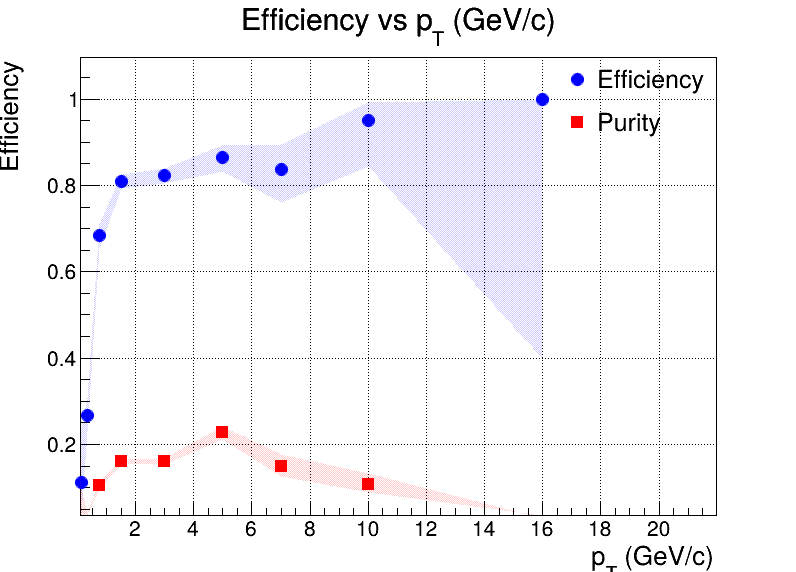
\includegraphics[width=\linewidth]{Combined_pt.png}
    \subcaption{Efficiency \& purity vs $p_T$}
    \label{fig:var-pt}
  \end{subfigure}\hfill
  \begin{subfigure}[t]{0.32\textwidth}
    \centering
    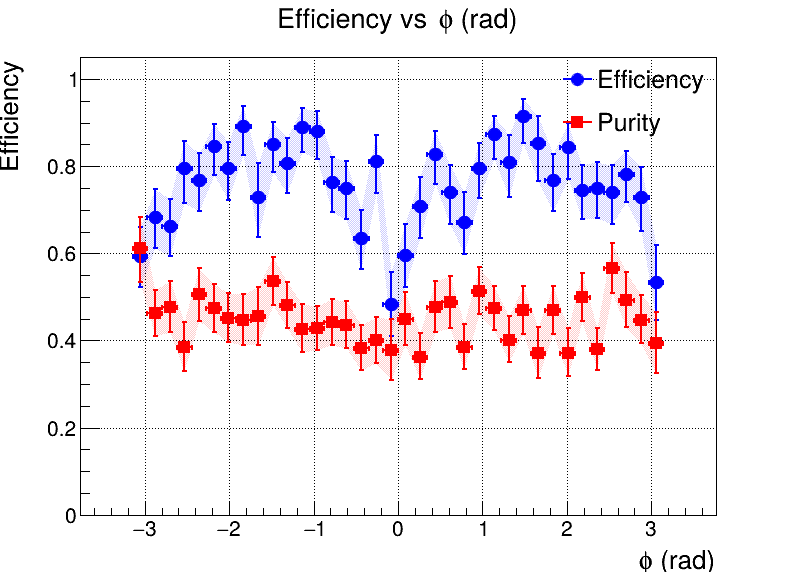
\includegraphics[width=\linewidth]{Combined_phi.png}
    \subcaption{Efficiency \& purity vs $\phi$}
    \label{fig:var-phi}
  \end{subfigure}\hfill
  \begin{subfigure}[t]{0.32\textwidth}
    \centering
    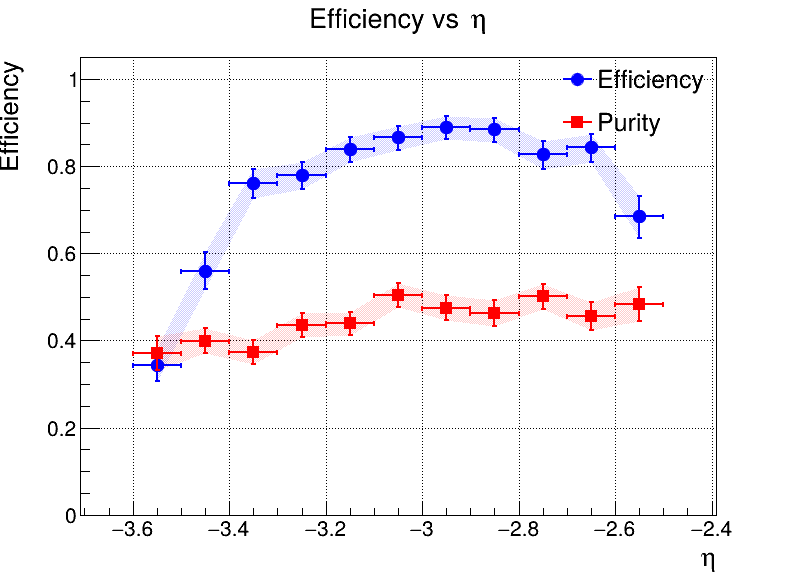
\includegraphics[width=\linewidth]{Combined_eta.png}
    \subcaption{Efficiency \& purity vs $\eta$}
    \label{fig:var-eta}
  \end{subfigure}

  \vspace{0.75em}

  % Row 2: two side by side (a bit wider)
  \begin{subfigure}[t]{0.48\textwidth}
    \centering
    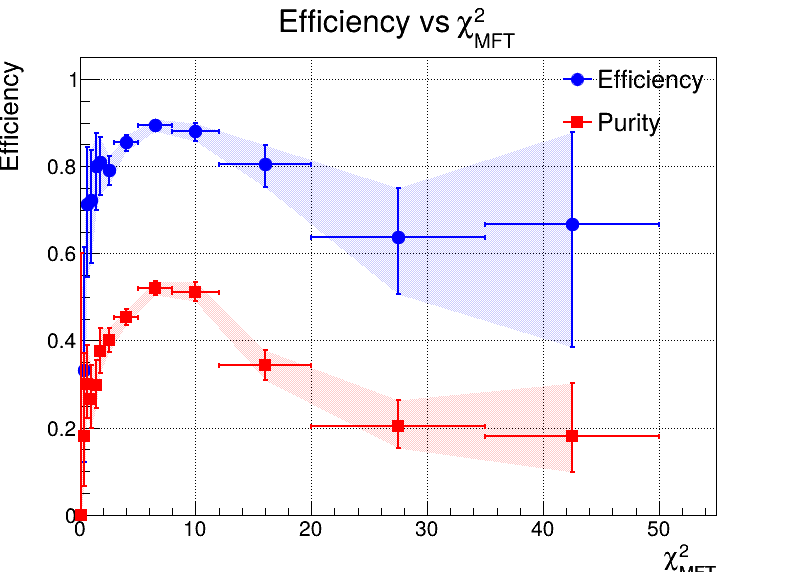
\includegraphics[width=\linewidth]{Combined_chi2_MFT.png}
    \subcaption{Efficiency \& purity vs matching $\chi^2$}
    \label{fig:var-chi2}
  \end{subfigure}\hfill
  \begin{subfigure}[t]{0.48\textwidth}
    \centering
    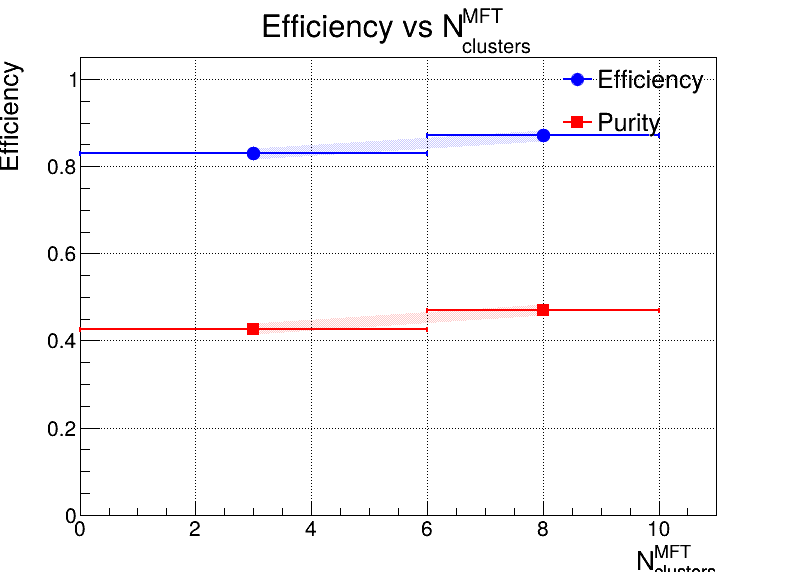
\includegraphics[width=\linewidth]{Combined_nClusters_MFT.png}
    \subcaption{Efficiency \& purity vs MFT cluster count}
    \label{fig:var-nclusters}
  \end{subfigure}

  \caption{Differential performance metrics for the matching algorithm across key variables.}
  \label{fig:differential-variables}
\end{figure}



Overall, the distributions confirm that efficiency remains relatively stable across most of the phase space, while purity exhibits stronger dependence--particularly in regions of low pT and extreme $\eta$, where combinatorial background is more pronounced.

\subsection{Optimization Studies}

The $\chi^2$ threshold plays a key role in balancing efficiency and purity \cref{sub@fig:opt-prod}. If the cut is set too tight, many true matches are lost, 
which lowers efficiency. If it is too loose, more fake matches are included, which reduces purity.
To find the best compromise, we scanned different values of the threshold \cref{sub@fig:opt-scan}.

\begin{figure}[H]
  \centering
  \begin{subfigure}[t]{0.48\textwidth}
    \centering
    
\includegraphics[width=\linewidth]{/Chi2Optimization.png}
    \subcaption{$\epsilon \times P$ vs $\chi^2$ threshold}
    \label{fig:opt-prod}
  \end{subfigure}\hfill
  \begin{subfigure}[t]{0.48\textwidth}
    \centering
    
\includegraphics[width=\linewidth]{/Chi2Scan_EffPur.png}
    \subcaption{$\epsilon$ and $P$ vs $\chi^2$ threshold}
    \label{fig:opt-scan}
  \end{subfigure}

  \caption{Optimization of the matching $\chi^2$ threshold: summary product and separate curves.}
  \label{fig:optimization}
\end{figure}



\subsection{Statistical Limitations}

The precision of these results is limited by the size of the Monte Carlo sample. This is most visible in regions where only a small number of tracks are available, such as high $p_T$ or large $\chi^2$ values. In these bins, the denominators used for efficiency or purity calculations are very small, which causes the statistical error bars to grow large. The effect does not indicate a problem with the matching algorithm or the detector, but simply reflects the limited statistics in those corners of phase space.

By contrast, in regions where many tracks are available--such as mid-$p_T$ or central $\eta$--the error bars remain small and the results are statistically robust. Increasing the size of the simulated dataset would reduce these fluctuations and provide more reliable estimates, especially in the high-$p_T$ and high-$\chi^2$ regions.

\section{Conclusion}

In this report, we studied the performance of the MFT--MCH track matching in terms of efficiency and purity. Using Monte Carlo simulations, we first extracted integrated values and then explored how the performance changes with key variables such as transverse momentum, azimuthal angle, pseudorapidity, matching $\chi^2$, and the number of MFT clusters.

The integrated results gave an efficiency of about 75\% and a purity of about 45\%. Differential studies showed that efficiency remains high across most of the phase space, while purity is more sensitive, especially at low $p_T$ and at looser $\chi^2$ selections. By scanning the $\chi^2$ threshold, we identified an optimal working point around $\chi^2 \approx 20$, which provides the best balance between efficiency and purity.

The main limitation of the study comes from the relatively small simulation sample, which leads to large statistical uncertainties at high $p_T$ and large $\chi^2$ values. Increasing statistics would allow for more reliable measurements in those regions and enable more detailed studies, for example in two dimensions.

Overall, the results confirm that the current matching approach performs well and is consistent with expectations.


\section{Code Availability}
The ROOT/C++ analysis framework developed for this study is maintained in a public GitHub repository: \url{https://github.com/haidaara/ALICE-O2-forward-track-analysis}. 
%*--------------------------------------------------*


\nocite{*}
\printbibliography

\end{document}